
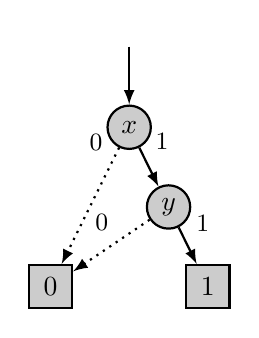
\begin{tikzpicture}[%
                costnode/.style={pos=0.6,rectangle,thick,
                                inner sep=2pt,draw,fill=white,text=black,font=\normalsize},%
                decisionnode/.style={circle,thick,minimum size=4mm,
                                inner sep=2pt,draw,fill=white!80!black,text=black,font=\normalsize},%
                xscale=2,yscale=1.35,>=latex]
        \node[] (before) at (0,2.35) {}; % incoming edge_value
        \node[decisionnode, minimum size=0.55cm] (x) at (0,1.5) {$x$};
        \node[decisionnode, minimum size=0.55cm] (y) at (0.25,0.75) {$y$};
        \node[draw,thick,fill=white!80!black,rectangle, minimum size=0.55cm]
        (after0) at (-0.5,0) {{$0$}};
        \node[draw,thick,fill=white!80!black,rectangle, minimum size=0.55cm]
        (after1) at (0.5,0) {{$1$}};
        \draw[->, thick] (before) to (x);
        % x =>
        \draw[->, thick, dotted] (x) to[bend right=0,label distance=0mm,edge
        label={\small{$0$}},swap,pos=0.1] (after0);
        \draw[->, thick] (x) to[bend left=0,label distance=0mm,edge
        label={\small{$1$}},pos=0.3] (y);
        % y =>
        \draw[->, thick, dotted] (y) to[bend right=0,label distance=0mm,edge
        label={\small{$0$}},swap,pos=0.4] (after0);
        \draw[->, thick] (y) to[bend left=0,label distance=0mm,edge
        label={\small{$1$}},pos=0.4] (after1);
\end{tikzpicture}
